\section{Theorie}
\label{sec:theorie}

Als Interferenz wird die Eigenschaft von Licht bezeichnet, bei Überlagerung die Amplitude zu ändern.
Dabei werden die Amplituden zweier oder mehrerer Wellen addiert.\\
Die Interferometrie nutzt diese Eigenschaft, um das Licht selbst zu untersuchen oder um materialspezifische Eigenschaften von Materie zu analysieren.

\subsection{Kohärenz}
Um Interferenz effektiv auszunutzen, ist es nötig die Kohärenz des Lichts zu betrachten.
Licht ist dann kohärent, wenn sich die Auslenkungen der Wellen, bis auf einen konstanten Phasenunterschied, zeitlich an verschiedenen Orten gleich ändern.
Zusätzlich muss die Wellenlänge aller individuellen Wellenpakete gleich sein.\\
\newline
Bei zeitlicher Kohärenz bleibt die Phasendifferenz in Ausbreitungsrichtung konstant, was durch die Kohärenzzeit $\tau_c$ bestimmt ist.
Diese gibt an, ab welchem Zeitpunkt die Phasendifferenz nicht mehr konstant bleibt und die Kohärenz sinkt.
Für die Kohärenzzeit $\tau_c$ gilt:
\begin{equation}
    \tau_c = \frac{1}{\Delta \nu} \qquad \text{mit} \qquad \Delta \nu \equiv \text{Bandbreite des Lichts}
\end{equation}
\newline
Bei räumlicher Kohärenz hat die Lichtwelle zum gleichen Zeitpunkt an verschiedenen Orten dieselbe Amplitude.\\
In \autoref{fig:coherencea} und \ref{fig:coherenceb} wird graphisch der Unterschied zwischen zeitlicher und räumlicher Kohärenz dargestellt.

\begin{figure}[H]
    \begin{subfigure}{.5\textwidth}
        \centering
        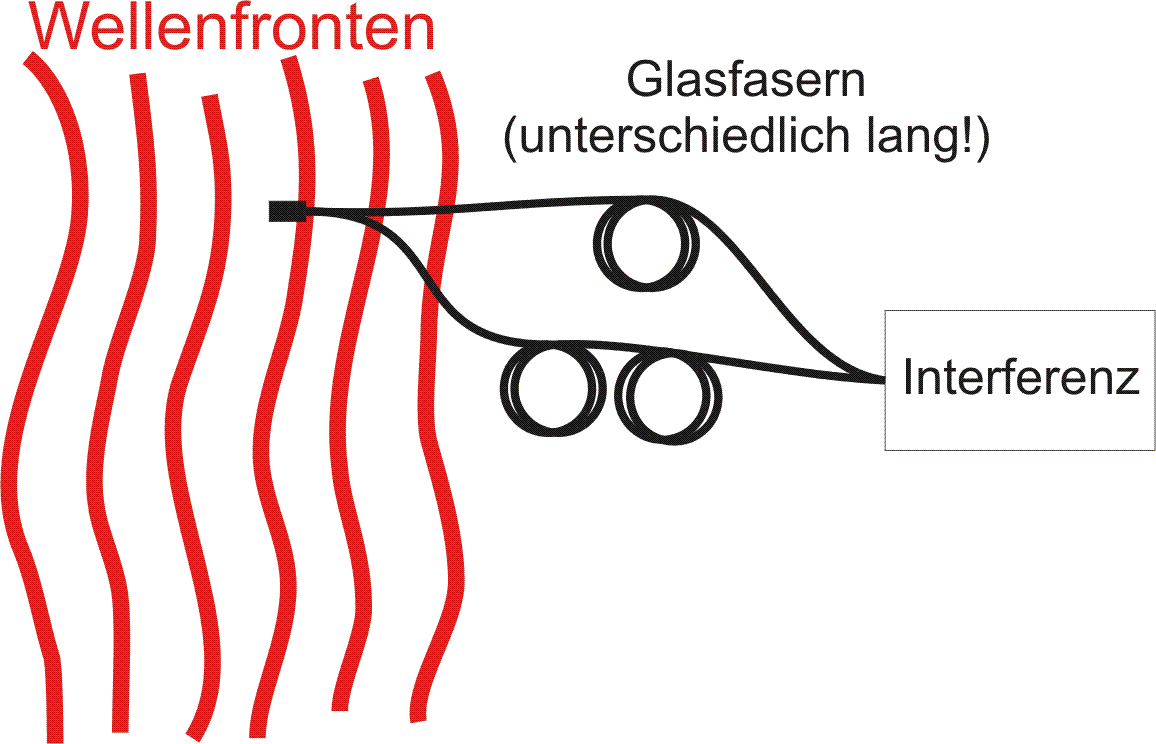
\includegraphics[scale=0.15]{images/zeitco.png}
        \caption{Darstellung von zeitlicher Kohärenz.\cite{koharenz}}
        \label{fig:coherencea}
    \end{subfigure}
    \begin{subfigure}{.5\textwidth}
        \centering
        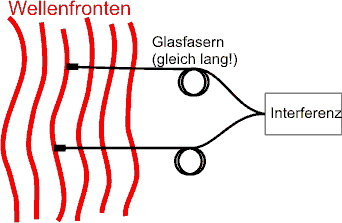
\includegraphics[scale=0.5]{images/raumco.png}
        \caption{Darstellung von räumlicher Kohärenz.\cite{koharenz}}
        \label{fig:coherenceb}
    \end{subfigure}
\end{figure}

Zusätzlich zur Kohärenzzeit lässt sich die Kohärenz auch mit einem Kontrast $V$ des Interferenzmusters beschreiben.
Bei maximalem Kontrast ist das Licht vollständig kohärent, bei Minimalem vollständig inkohärent.
Der Kontrast berechnet sich aus den Intensitäten des Lichts und dem Kohärenzgrad
\begin{equation}
    \Gamma = \langle E_1 E_2^\dagger \rangle \quad \text{,} \quad \gamma = \frac{\Gamma}{\sqrt{I_1 I_2}},
    \label{eq:grad}
\end{equation}
und es gilt:
\begin{equation}
    V = \frac{2\sqrt{I_1I_2}}{I_1 + I_2}|\gamma|
    \label{eq:kontrast_formel}
\end{equation}
Wird vollständig kohärentes Licht angenommen, gilt für den Kontrast auch \autoref{eq:kontrast}.
\begin{equation}
    V = \frac{I_{\text{max}} - I_{\text{min}}}{I_{\text{max}} + I_{\text{min}}}
    \label{eq:kontrast}
\end{equation}
Vollständig kohärentes Licht ist praktisch nicht umsetzbar, da Lichtquellen nicht eindeutig monochromatisch leuchten.
Da es nur teilmonochromatisches Licht gibt, gibt es dahingehend auch nur Teilkohärenz.

\subsection{Fresnel-Arago-Gesetze}
Die Fresnel-Arago-Gesetze befassen sich mit der Polarisation des Lichts bei Interferenz.\\
Licht ist in der Regel unpolarisiert und wird deswegen in einen senkrechten und horizontalen Polarisationsanteil aufgespalten.
Auch für polarisiertes Licht mit integrierter Phasenverschiebung, wie zum Beispiel zirkulär polarisiertem Licht, ist das möglich, wobei die Phasenverschiebung erhalten bleibt.\\
Die vier Gesetze von Augustin Jean Fresnel und François Arago befassen sich mit zwei Lichtstrahlen und deren Polarisation zueinander, um deren Interferenz zu bestimmen.
Sie lauten zusammengefasst:
\begin{itemize}
    \item Zwei linear polarisierte Lichtstrahlen mit zueinander parallelen Polarisationsebenen, interferieren wie nicht polarisiertes Licht.
    \item Zwei linear polarisierte Lichtstrahlen mit zueinander senkrechten Polarisationsebenen, interferieren nicht.
    \item Zwei zueinander senkrecht linear polarisierte Lichtstrahlen, interferieren nur dann, wenn sie aus einem Strahl kamen und erneut zu einem Strahl mit selber Polarisationsebene zusammengeführt werden.
    \item Zwei zueinander senkrecht linear polarisierte Lichtstrahlen, interferieren bei Zusammenführung nicht, wenn sie aus nicht polarisiertem Licht entstanden sind.\cite{fresnel}
\end{itemize}

\subsection{Intensitäten und Interferenzbild}
Um den Kontrast theoretisch zu berechnen, müssen die Intensitäten $I_{\text{max,min}}$ bekannt sein.
Sie sind definiert als benachbarte Intensitäten der konstruktiven und destruktiven Interferenz und werden bestimmt durch
\begin{equation}
    I_{\text{max,min}} \propto I_{\text{Laser}}\left[1 \pm 2\cos\left(\phi\right)\sin\left(\phi\right)\right],
    \label{eq:intense}
\end{equation}
wobei $I_{\text{Laser}}$ die mittlere Ausgangsintensität des He-Ne Lasers und $\phi$ der Winkel des Polarisationsfilters vor dem Interferometer ist.
\autoref{eq:intense} kann aus der Beziehung
\begin{equation}
    I \propto <|E_1\cos\left(\omega t\right) + E_2\cos\left(\omega t + \delta\right)|^2>
\end{equation}
hergeleitet werden.
Hierbei sind $E_{1,2}$ die Amplituden der elektrischen Felder der Lichtstrahlen im Interferometer, $<...>$ eine Zeitmittlung über eine Periode und $\delta$ die Phasendifferenz der beiden Strahlen.\\
Wird angenommen, dass beide Strahlen dieselbe Amplitude $E$ aufweisen, so lassen sich $E_{1,2}$ anhand des Polarisationswinkels $\phi$ ausdrücken:
\begin{align}
    E_1 = E\cdot \cos\left(\phi\right)\\
    E_2 = E\cdot \sin\left(\phi\right)
\end{align}
Die Abhängigkeit des Kontrasts vom Polarisationswinkel ist gegeben durch
\begin{equation}
    V = \sin\left(2\phi\right)
    \label{eq:abhang}
\end{equation}
und kann ermittelt werden, indem \autoref{eq:intense} in \autoref{eq:kontrast} eingesetzt wird.\\
\autoref{eq:abhang} zeigt auf, dass der Kontrast für die Polarisationswinkel $\phi = \SI{45}{\degree}$ und $\phi = \SI{135}{\degree}$ maximal ist.\\
\newline
Für die Justage des Interferometers, wird das Interfernzbild betrachtet.
Sind mehrere Interferenzstreifen zu erkennen, also mehrere Intensitätsmaxima und -minima als Streifen im Bild, so ist das Interometer nicht korrekt justiert.
Das Interferenzbild soll vollständig ein Intensitätsmaximum beziehungsweise ein Intensitätsminimum ergeben, für die korrekte Ausführung, der in \autoref{sec:durchfuehrung} beschriebenen Schritte.\\
Die Detektion der Intensitäten erfolgt mittels zwei Photodioden, dessen Differenz genutzt wird, um klare Nulldurchgänge des Signals zu messen.
Die Differenz bei Übergängen eines Maximums zu einem Minimum ist hoch, sodass diese genauer ist als die Analyse von den einzelnen Signalen.

\subsection{Berechnung von Brechungsindizes}
Im Verlauf der Messungen werden die Brechungsindizes von Glas und Luft bestimmt.
\subsubsection{Brechungsindex von Glas}
Für die Phasenverschiebung von Glas gilt in Kleinwinkelnäherung mit dem Drehwinkel $\Theta$
\begin{equation}
    \Delta\Phi\left(\Theta\right) = \frac{2\pi}{\lambda_{\text{vac}}}T\left(\frac{n - 1}{2n}\Theta^2 + \mathcal{O}\left(\Theta^4\right)\right).
    \label{eq:poli}
\end{equation}
Für die Anzahl der Intensitätsmaxima und -Minima gilt
\begin{equation}
    M = \frac{\Delta\Phi\left(\Theta\right)}{2\pi}
\end{equation}
, sodass die Anzahl $M$ berechnet werden kann mit
\begin{equation}
    M = \frac{T}{\lambda_{\text{vac}}}\left(\frac{n - 1}{2n}\Theta^2 + \mathcal{O}\left(\Theta^4\right)\right).
    \label{eq:brechungint}
\end{equation}
Hierbei ist $T = \SI{1}{\milli\metre}$ die Dicke der Glasplatte, $\lambda_{\text{vac}}$ die Wellenlänge im Vakuum und $n$ der Brechungsindex.\\
Im Strahlengang des Interferometers ist für je einen Strahl ein Glasplättchen verbaut, sodass insgesamt zwei in der Halterung verbaut sind.
Zusätzlich sind die Plättchen um $\Theta_0 = \pm \SI{10}{\degree}$ angewinkelt, also $+\SI{10}{\degree}$ für den einen Strahl und $-\SI{10}{\degree}$ für den anderen.
Daher gilt für die zwei separaten Drehwinkel:
\begin{equation}
    \Theta_{\text{hor,ver}} = \pm\Theta_0 + \Delta\Theta
\end{equation}
In die \autoref{eq:brechungint} eingesetzt ergibt dies:
\begin{equation}
    M = \frac{T}{\lambda_{\text{vac}}}\left(\frac{n - 1}{2n}|\Theta_{\text{hor}}^2 - \Theta_{\text{ver}}^2|\right) \quad \iff \quad M = \frac{T}{\lambda_{\text{vac}}}\cdot\frac{n - 1}{2n}|4\Theta_0 \Delta\Theta|
\end{equation}
Umgestellt nach dem Brechungsindex $n$ ergibt sich
\begin{equation}
    n = \frac{1}{1 - \frac{2\lambda_{\text{vac}}M}{T|4\Theta_0\Delta\Theta|}}
    \label{eq:brechungsindex}
\end{equation}
Somit ist der Brechungsindex abhängig von der Intensitätsanzahl $M$ und dem gedrehten Winkel der Glasplättchen $\Delta\Theta$.
\subsubsection{Brechungsindex von Luft}
Die für die Bestimmung des Brechungsindexes von Luft benötigte Gaszelle hat eine Länge von $L = \SI{100.0\pm0.1}{\milli\metre}$ und trägt aufgrund der verbauten Optiken zu einer Phasenverschiebung von
\begin{equation}
    \Delta\Phi = \frac{2\pi}{\lambda_{\text{vac}}}\Delta nL \quad \iff \quad M = \frac{\Delta nL}{\lambda_{\text{vac}}}
    \label{eq:gasphase}
\end{equation}
bei, verglichen mit einem Strahl, der nicht durch die Gaszelle propagiert.\\
Der Brechungsindex von Gasen wird durch das Lorentz-Lorenz-Gesetz approximiert, welches den Brechungsindex abhängig von Gasdruck $p$ und Gastemperatur $T$ angibt.
Es lautet:
\begin{equation}
    n \approx \sqrt{1 + \frac{3Ap}{RT}}
    \label{eq:lorentz}
\end{equation}
Hierbei ist $R$ die allgemeine Gaskonstante und $A$ die Molrefraktion, die definiert ist über
\begin{equation}
    A = \frac{4\pi}{3}N_A\alpha
\end{equation}
mit der Avogadro-Konstante $N_A$ und der durchschnittlichen Polarisierbarkeit $\alpha$.